\begin{center}
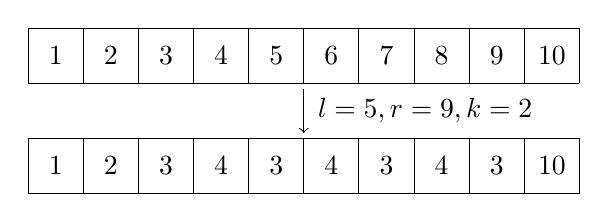
\begin{tikzpicture}[xscale=0.7, yscale=-0.7]

\draw (0,0) grid (10,1);
\node at (0.5,0.5) {$1$};
\node at (1.5,0.5) {$2$};
\node at (2.5,0.5) {$3$};
\node at (3.5,0.5) {$4$};
\node at (4.5,0.5) {$5$};
\node at (5.5,0.5) {$6$};
\node at (6.5,0.5) {$7$};
\node at (7.5,0.5) {$8$};
\node at (8.5,0.5) {$9$};
\node at (9.5,0.5) {$10$};

\draw[arrows={->}] (5, 1.1) -- (5, 1.9);
\node at (7.2, 1.5) {$l = 5, r = 9, k = 2$};

\draw (0,2) grid (10,3);
\node at (0.5,2.5) {$1$};
\node at (1.5,2.5) {$2$};
\node at (2.5,2.5) {$3$};
\node at (3.5,2.5) {$4$};
\node at (4.5,2.5) {$3$};
\node at (5.5,2.5) {$4$};
\node at (6.5,2.5) {$3$};
\node at (7.5,2.5) {$4$};
\node at (8.5,2.5) {$3$};
\node at (9.5,2.5) {$10$};

\end{tikzpicture}
\captionof{figure}{Ejemplo de operación tipo 2}
\end{center}